Considering difference multisets over an arbitrary abelian group one can notice that some of the surfaces defined by our equations are always the same. There is always the hyperplane $\sum {n_\mu} = k$ and the hypersphere $\sum n_\mu^2 = k + \lambda$ centered at the origin (see Figure \ref{general:figure:surfaces}). 

The second equation confines every multiplicity: $n_\mu \leq \sqrt{k+\lambda}$. By investigating the intersection more thoroughly we discover that the multiplicities are actually bound to be near to their average $k/v$.

\begin{figure}
	\centering
	\begin{subfigure}[b]{0.5\textwidth}
		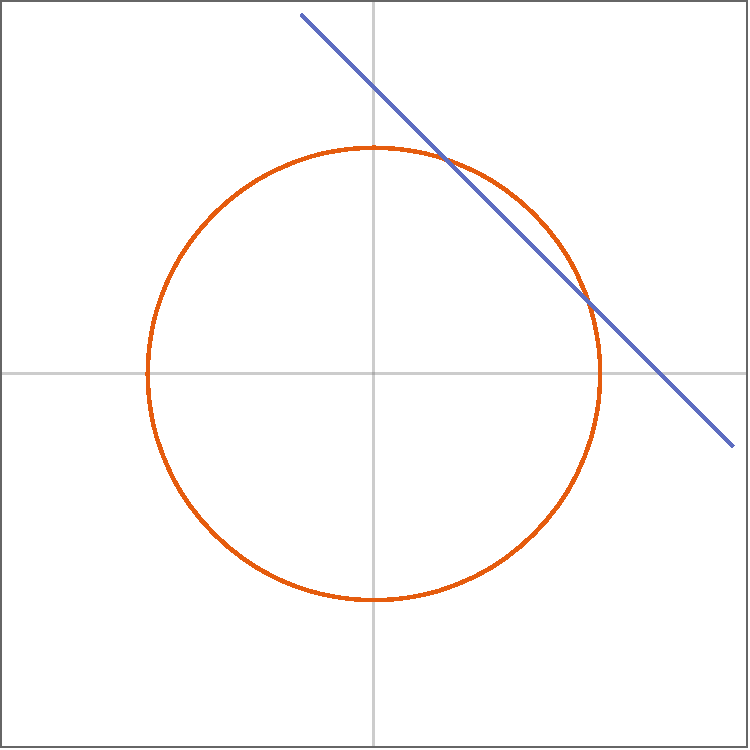
\includegraphics[width=\textwidth]{assets/surfacesIn2D}
	\end{subfigure}%
	~
	\begin{subfigure}[b]{0.5\textwidth}
		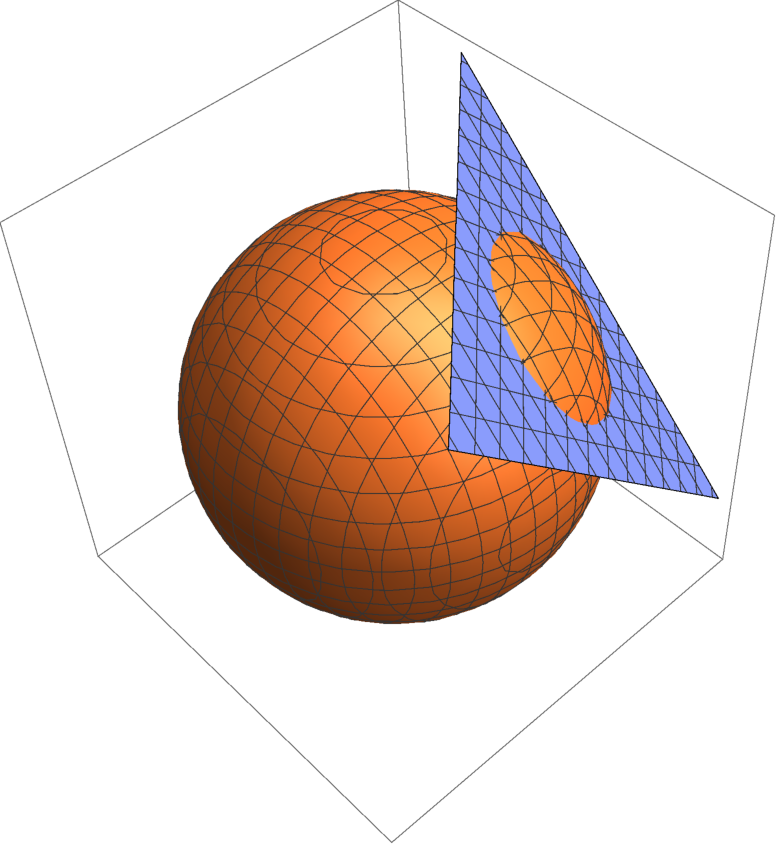
\includegraphics[width=\textwidth]{assets/surfacesIn3D}
	\end{subfigure}
	\caption{The $\sum {n_\mu} = k$ and $\sum n_\mu^2 = k + \lambda$ surfaces in two and three dimensions.}
	\label{general:figure:surfaces}
\end{figure}
	
\begin{theorem}
	\label{general:theorem:limits}
	If $M$ is a $(G,k)$-difference multiset and $|G|=v$ then
	\begin{equation}
		\forall \gamma \in G \colon\qquad \frac{k-(v-1)\sqrt k}{v} \leq n(\gamma,M) \leq \frac{k+(v-1)\sqrt k}{v}
	\end{equation}
\end{theorem}

\begin{proof}
	Take equation \eqref{apparatus:eq:system} for the identity element and equation \eqref{apparatus:eq:ni} as constraints:
	
	\begin{equation}
		\begin{cases}
			\sum {n_\mu} = k \\
			\sum (n_\mu(n_\mu-1)) = \lambda.
		\end{cases}
	\end{equation}
	
	Let us optimize $n_\gamma=n(\gamma,M)$ respecting the constraints. Add the first equation to the second and move all the terms to the left hand side:
	
	\begin{equation}
		\begin{cases}
			k - \sum {n_\mu} = 0 \\
			k + \lambda - \sum n_\mu^2 = 0.
		\end{cases}
	\end{equation}
	
	We apply the method of Lagrange multipliers to obtain the maximum and minimum of $n_\gamma$. 
	
	We use the following Lagrange function ($\lambda_1$ and $\lambda_2$ here is the standard Lagrange multiplier notation and have nothing in common with the parameter $\lambda$).
	
	\begin{equation}
		\mathcal L = n_\gamma - \lambda_1 (k - \sum n_\mu) - \lambda_2 (k + \lambda - \sum n_\mu^2)
	\end{equation}
	
	By a standard application of this method the bounds of the theorem statement are obtained. We omit the routine calculations.
\end{proof}

Theorem \ref{general:theorem:limits} suggests using digressions instead of multiplicities (thus simplifying the equations) and greatly reduces the amount of options for every $n_\gamma$. This simplification allows decent computer searches which enabled us to discover some of the patterns that led to results presented in this paper.
	
\begin{figure}
	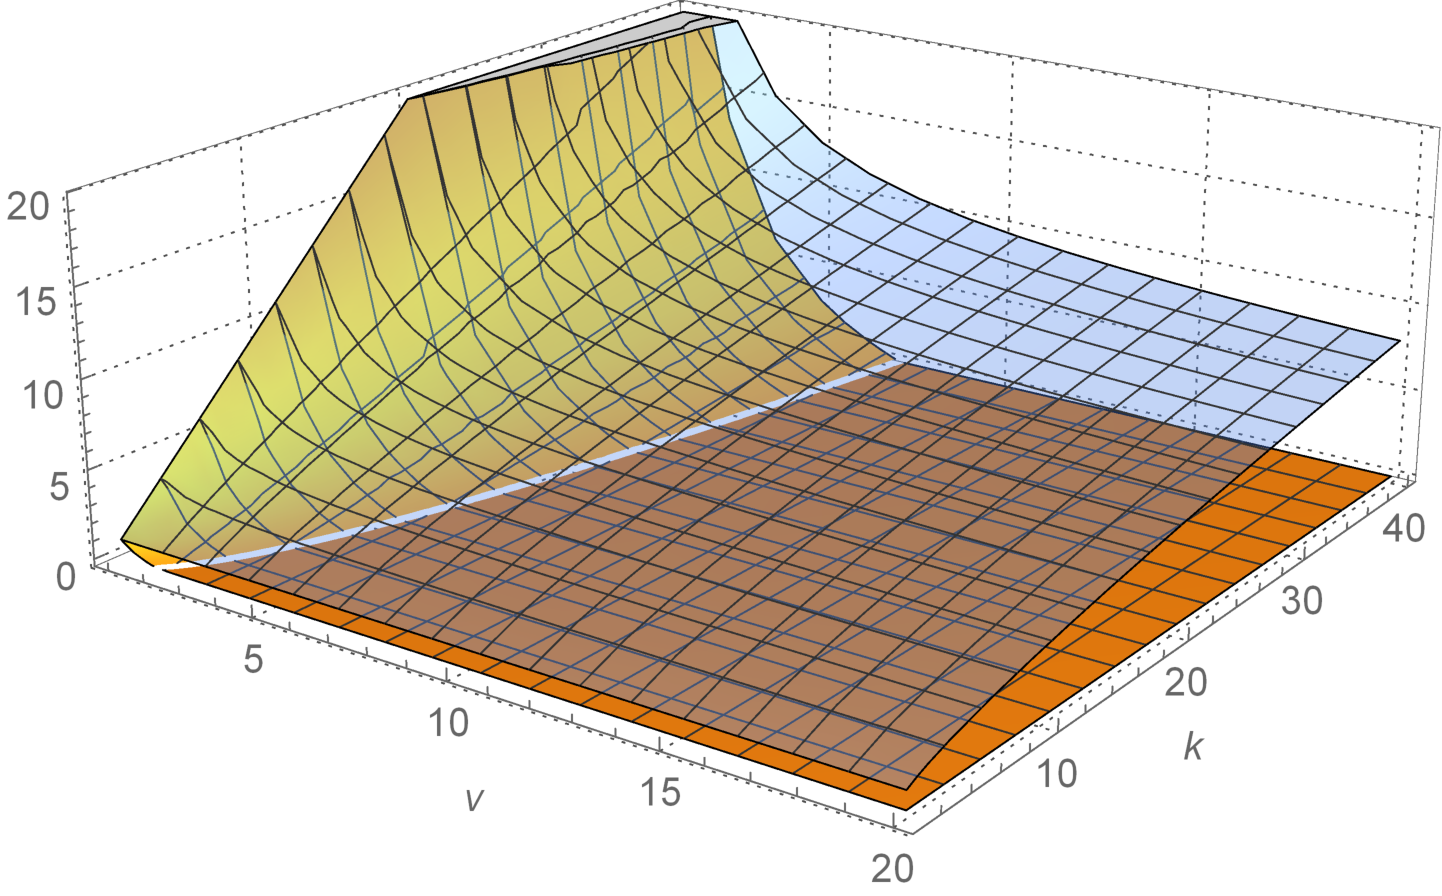
\includegraphics[width=\textwidth]{assets/boundingSurfaces}
	\caption{Lower and upper bounds for the values of $n_\gamma$ with respect to $v$ and $k$.}
	\label{general:figure:limits}
\end{figure}
